

With our formulation for the expected percentage of points appearing on a
slice, $\exppts{r}$, we now turn to the derivation of the expected
number of fragments that need to be drawn per point on a slice, 
$\expfrags$. Only the points which pass the filtering stage of our algorithm
are taken into account at this point. 
To do this,
we derive the expected area of 
the quad each point will create on the slice given that the point is a certain
distance, $t$, from the slice. Even though each point drawn
leaves a circular splat, we still must process it as a quad since the GPU
does not support circle primitives. To discard a sample point we generate a
quad of area $0$.
%For convenience, in the derivation below we drop
%the functional notation, $\expfrags$ in favor of the more compact
%$E[q]$.

\section{Expected number of fragments}

Given that we need to draw a particular data point, the question is how large
an impact in terms of number of fragments does it make on the 2D slice. As the
distance from a sample point to the slice, $t$, increases the area of the 
quad, $q$, decreases. This is due to the slice passing through a smaller area 
of the
hyperspherical kernel surrounding the data point. \autoref{fig:circle} shows the
relationship between $t$ and the half-length of one of the sides of the 
quad $u$.  In \autoref{fig:circle}, (as usual) $r$ is the maximum search distance.

\begin{figure}[htb]
\centering
\begin{subfigure}{0.4\textwidth}
  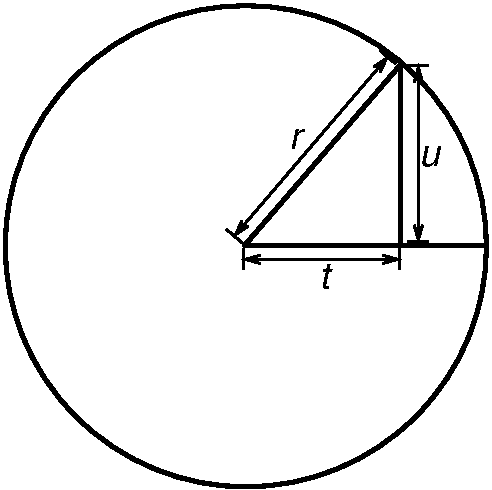
\includegraphics[width=\textwidth]{circle_diagram}
  \caption{
  }
  \label{fig:circle}
\end{subfigure}%
\begin{subfigure}{0.4\textwidth}
  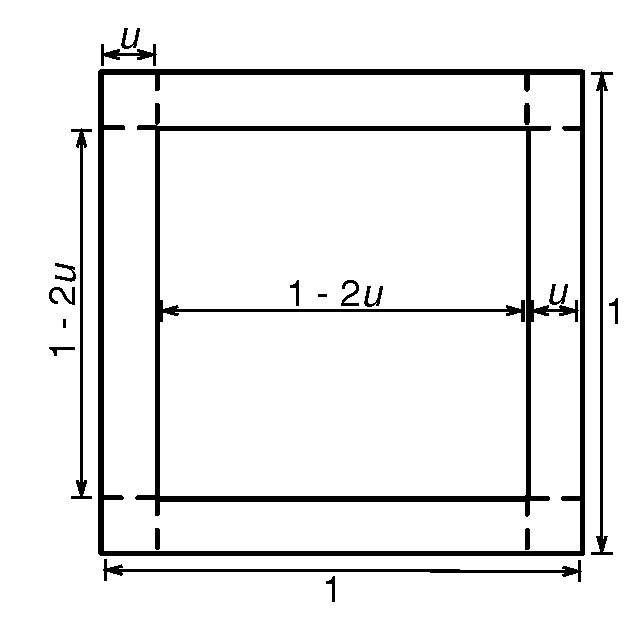
\includegraphics[width=\textwidth]{box_probs}
  \caption{
  }
  \label{fig:quad_size}
\end{subfigure}
\caption[Kernel/slice interaction]{
  (a) A 2D cross-section of a hypersphere of radius $r$ representing 
  the spherical kernel 
  centred around a particular sample point.  The slice we are
  viewing intersects the kernel at a distance, $t$, away.  This 
  creates an impression of side length $2u = 2\sqrt{r^2-t^2}$ on the 
  slice.  We need to draw a quad on screen for this impression.
  (b) shows the possible regions on the slice (the outer square)
  in which the center of the sample point lies.  If the sample point
  does not lie in the center region then some of the quad will be clipped
  by the edges of the screen and we will not have to render as many 
  fragments.
}
\label{fig:appendix_geom}
\end{figure}

Therefore, $u$ is related to $t$ through
\begin{align}
  u &= \sqrt{r^2-t^2} \label{eq:u_to_t}
\end{align}
and the
maximum area of the quad is $4u^2$.  However, the quad size is not always
$4u^2$.   If the center of the quad is within $u$ of the edge of the slice
then the quad will be clipped and it will be smaller than $4u^2$.
This ``maximum size'' area is the inner square in \autoref{fig:quad_size}.
We can formulate the expected quad size as a function of $u$: $E[q](u)$.
To find $E[q](u)$ we must integrate the quad size given a location on 
the slice $(x,y)$ over all possible positions of sample points,
\begin{align*}
  E[q](u) &= \int_{x=0}^1 \int_{y=0}^1 q(x, y, u) \, dy \, dx
  \text{.}
\end{align*}

Note that there are three regions on the slice a point may fall in,
the probability of the point falling into each region is a direct result
of the area of each region:

\begin{itemize}
\item \textbf{corner:} where the quad size ranges from $u^2$ to $4u^2$
                    with probability $P = 4u^2$
\item \textbf{side:}   where the quad size ranges from $2u^2$ to $4u^2$ 
                    with probability $P = 4u(1-2u)$
\item \textbf{center:} where the quad size is $4u^2$
                    with probability $P = (1-2u)^2$
\end{itemize}

Therefore, our formulation for $E[q](u)$ can be split into 3 integrals:
\begin{align*}
  E[q](u) &=   4 \int_{x=0}^u \int_{y=0}^u (x+u)(y+u) \, dy \, dx     \\
           & + 4 \int_{x=u}^{1-u} \int_{y=0}^u (2u)(y+u) \, dy \, dx \\
           & + \int_{x=u}^{1-u} \int_{y=u}^{1-u} 4u^2 \, dy \, dx    \\
          &= 4A + 4B + C
          \text{.}
\end{align*}

Where $A$, $B$, and $C$ are the corner, side, and center cases respectively.
We solve each integral individually:
\begin{align*}
  A &= \int_{x=0}^{u} \int_{y=0}^{u} (x+u)(y+u) \, dy \, dx \\
    &= \int_{x=0}^{u} (x+u) \int_{y=0}^{u} (y+u) \, dy \, dx \\
    &= \int_{x=0}^{u} (x+u) \left(\left. \frac{y^2}{2} + uy \right|_0^u \right) \, dx \\
    &= \int_{x=0}^{u} (x+u) \left(\frac{3u^2}{2} \right) \, dx \\
    &= \frac{3u^2}{2} \left(\left. \frac{x^2}{2} + xu \right|_0^u \right) \\
  A &= \frac{9u^4}{4} 
  \text{,}
\end{align*}
\begin{align*}
  B &= \int_{x=u}^{1-u} \int_{y=0}^u (2u)(y+u) \, dy \, dx \\
    &= \int_{x=u}^{1-u} (2u) \int_{y=0}^u (y+u) \, dy \, dx \\
    &= 2u \int_{x=u}^{1-u} 
            \left(\left. \frac{y^2}{2} + yu\right|_0^u \right) \, dx \\
    &= 2u \int_{x=u}^{1-u} \left( \frac{u^2}{2}+u^2 \right) \\
    &= 2u (1-u-u) \frac{3u^2}{2} \\
    &= 2u (1-2u) \frac{3u^2}{2} \\
    &= (2u-4u^2) \frac{3u^2}{2} \\
  B &= 3u^3 - 6u^4 
  \text{,}
\end{align*}
and
\begin{align*}
  C &= \int_{x=u}^{1-u} \int_{y=u}^{1-u} 4u^2 \, dy \, dx \\
    &= (1-u-u) (1-u-u) (4u^2) \\
    &= (1-2u) (1-2u) (4u^2) \\
    &= (1-4u+4u^2) (4u^2) \\
  C &= 4u^2 - 16u^3 + 16u^4
  \text{.}
\end{align*}

Substituting $A$, $B$, and $C$ back into the formula we get,
\begin{align*}
  E[q](u) &= 4A + 4B + C \\
          &= 4 \frac{9u^4}{4} + 4 (3u^3 - 6u^4) + (4u^2 - 16u^3 + 16u^4) \\
          &= 9u^4 + 12u^3 - 24u^4 + 4u^2 - 16u^3 + 16u^4 \\
  E[q](u) &= 4u^2 - 4u^3 + u^4 \numberthis \label{eq:app:expfrags} \text{.}
\end{align*}

\section{Expected 3D quad size}

Now we can turn to a formulation of $\expfrags$ which is the expected quad
size over all $0 \le t \le r$.  We also need to take into account the
likelihood of a point lying at a particular value of $t$, which we
denote $P_t$:
\begin{align*}
  \expfrags = \int_0^r E[q](u) P_t \, dt
  \text{.}
\end{align*}

There are 2 cases we need to consider, the $d=3$ case and the $d>3$ case.
We first derive $\expfrags$ for the simpler $3D$ case in order to illustrate
the basic procedure combining the expected impact size with the number of
points drawn.

When $d=3$ all points lie on a line extending on either side of the slice.
Therefore, $P_t = 2$, which is also the surface area of a $1$-dimensional
sphere.
Since all distances are equally likely in this case, we can simply integrate
$E[q](u)$ over all $t$:
\begin{align*}
\expfrags 
     &= \int_{0}^r E[q] (u) P_t \, dt \\
     &= \int_{0}^r (4u^2 - 4u^3 + u^4) 2 \, dt \text{.}\\
\intertext{We can rewrite the formula in terms of $t$ by using \autoref{eq:u_to_t}}
     &= 2 \int_{0}^r 
          4(\sqrt{r^2-t^2})^2 - 4(\sqrt{r^2-t^2})^3 + (\sqrt{r^2-t^2})^4 \, dt
          \text{.}
\end{align*}

To make things easier to integrate we substitute $t$ with spherical coordinates:
\begin{align*}
t  &= r \sin \, \theta \\
dt &= r \cos \, \theta \, d\theta \\
\sqrt{r^2 - t^2} &= r \cos \, \theta
\text{,}
\end{align*}
which leads to
\begin{align*}
\expfrags &= 2 \int_{0}^{\pi/2}
          \left(4(r\cos\,\theta)^2 
              - 4(r\cos\,\theta)^3 
              + (r\cos\,\theta)^4
          \right)
        r\cos\,\theta\,d\theta \\
     &= 2 \int_{0}^{\pi/2}
          4r^3\cos^3\,\theta 
        - 4r^4\cos^4\,\theta 
        + r^5\cos^5\,\theta \, d\theta \\
     &= 8r^3 \int_{0}^{\pi/2} \cos^3\,\theta d\theta
      - 8r^4 \int_{0}^{\pi/2} \cos^4\,\theta d\theta
      + 2r^5 \int_{0}^{\pi/2} \cos^5\,\theta \, d\theta \\
     &= \left. 8r^3 \left(
            \frac{\cos^2\,\theta\,\sin\,\theta}{3}
          + \frac{2}{3} \int \cos\,\theta d\theta \right)
        \right|_{0}^{\pi/2} \\
     &\qquad 
      - \left. 8r^4 \left(
            \frac{\cos^3\,\theta\,\sin\,\theta}{4}
          + \frac{3}{4} \int \cos^2\,\theta d\theta \right)
        \right|_{0}^{\pi/2} \\
     &\qquad
       + \left. 2r^5 \left(
            \frac{\cos^4\,\theta\,\sin\,\theta}{5}
          + \frac{4}{5} \int \cos^3\,\theta d\theta \right)
        \right|_{0}^{\pi/2} \\
     &= \left. 8r^3 \left(
            \frac{\cos^2\,\theta\,\sin\,\theta}{3}
          + \frac{2}{3} \sin\,\theta \right)
        \right|_{0}^{\pi/2} \\
     &\qquad
       - \left. 8r^4 \left(
            \frac{\cos^3\,\theta\,\sin\,\theta}{4}
          + \frac{3}{4} \left(
                \frac{\theta}{2}
              + \frac{1}{4} \sin\,2\theta \right)
            \right)
        \right|_{0}^{\pi/2} \\
     &\qquad
       + \left. 2r^5 \left(
            \frac{\cos^4\,\theta\,\sin\,\theta}{5}
          + \frac{4}{5} \int \cos^3\,\theta d\theta \right)
        \right|_{0}^{\pi/2} \\
     &= 8r^3 \left(\frac{2}{3}\right)
      - 8r^4 \left(\frac{3\pi}{16}\right)
      + 2r^5 \left(\frac{8}{15} \right) \\
\expfrags &= \frac{16r^3}{3} - \frac{6\pi r^4}{4} + \frac{16r^5}{15}
\text{.}
\end{align*}


\section{Expected quad size for the $d>3$ case}

%\subsubsubsection{Identities}

When $d>3$, two of the dimensions are determined by the slice however the
sample point's position with respect to the remaining $(d-2)$-dimensions 
determine its distance to the slice.  All points with the same 
$(d-2)$-dimensional distance will have the same impact on the slice.
Therefore, we can view all points at distance $t$ as lying along the surface 
of a hyperball.  However, this hyperball may be clipped by the edges of the
parameter space so the likelihood of a point lying at distance $t$ is given
by the surface area of the clipped hypersphere at $t$.  Similar to a sphere,
this can be found by taking the derivative of \autoref{eq:exppts} with 
respect to $r$:
\begin{align*}
 S(t,d) 
   &= \frac{d \exppts{t}}{d t} \\
   &= \frac{d \left[
    \sum_{i=0}^{n} (-1)^{i} {n \choose i}
         \frac{\pi^{(n-i)/2}t^{n+i}}{\Gamma(\frac{n+i}{2} + 1)} 
 \right]}{dt} \\
   &= \sum_{i=0}^{n} (-1)^{i} {n \choose i}
         \frac{(n+i)\pi^{(n-i)/2}t^{n+i-1}}{\Gamma(\frac{n+i}{2} + 1)} \\
   &= \sum_{i=0}^{n} (-1)^{i} {n \choose i}
         \frac{2\pi^{(n-i)/2}t^{n+i-1}}{\Gamma(\frac{n+i}{2})} 
         \text{.}
\end{align*}
We then integrate this
together with the expected area of a quad (\autoref{eq:app:expfrags}) over
all $0 \le t \le r$ to find $\expfrags$:
\begin{align*}
\expfrags &= \int_0^r E[q](u) P_t \, dt \\
     &= \int_0^r (4u^2 - 4u^3 + u^4)
        \frac{S(t,d)}{\exppts{r}} \, dt \\
     &= \int_0^r 
        \left(4(\sqrt{r^2-t^2})^2 - 4(\sqrt{r^2-t^2})^3 + (\sqrt{r^2-t^2})^4\right)
        \frac{S(t,d)}{\exppts{r}} \, dt \\
     &= \frac{1}{\exppts{r}} \int_0^r 
        \left(4(\sqrt{r^2-t^2})^2 - 4(\sqrt{r^2-t^2})^3 + (\sqrt{r^2-t^2})^4\right)
        S(t,d) \, dt \\
     &= \frac{1}{\exppts{r}} \int_0^r 
        \left(4(\sqrt{r^2-t^2})^2 - 4(\sqrt{r^2-t^2})^3 + (\sqrt{r^2-t^2})^4\right) \\
     &\qquad\qquad\qquad
       \left(
           \sum_{i=0}^{n} (-1)^{i} {n \choose i}
               \frac{2\pi^{(n-i)/2}t^{n+i-1}}{\Gamma(\frac{n+i}{2})} 
        \right) \, dt 
        \text{.}
\end{align*}

Just to simplify the writing a bit we can replace the factors of the formula
that don't depend on $t$ by,
\begin{align*}
  K_i &= (-1)^i {n \choose i} \frac{2\pi^{(n-i)/2}}{\Gamma((n+i)/2)}
  \text{.}
\end{align*}
$K_i$ is the expected area of the hypersphere clipped by all possible
combinations of the $i$-dimensional space.  

With this substitution we get,
\begin{align*}
\phantom{\expfrags}
     \expfrags &= \frac{1}{\exppts{r}} \int_0^r 
        \left(4(\sqrt{r^2-t^2})^2 - 4(\sqrt{r^2-t^2})^3 + (\sqrt{r^2-t^2})^4\right) 
        \left(
          \sum_{i=0}^{n} K_i t^{n+i-1}
        \right) \, dt 
        \text{.}
\end{align*}

Rather than integrating over square roots, we can use trigonometric 
substitution to simplify the formula:
\begin{align*}
t  &= r \sin \theta \\
dt &= r \cos \theta \, d\theta \\
\sqrt{r^2 - t^2} &= \sqrt{r^2 - (r\sin \theta)^2} \\
                 &= r \cos \theta 
                 \text{.}
\end{align*}
Then we get,
\begin{align*}
\phantom{\expfrags}
     &= \frac{1}{\exppts{r}} \int_0^{\pi/2}
        \left(4(r\cos \theta)^2 - 4(r\cos \theta)^3 + (r\cos \theta)^4\right) \\
     &\qquad\qquad\qquad
        \left(
          \sum_{i=0}^{n} K_i (r\sin \theta)^{n+i-1} \right) 
        r\cos \theta \, d\theta \\
     &= \frac{1}{\exppts{r}} \int_0^{\pi/2}
        \left(4r^3\cos^3 \theta - 4r^4\cos^4 \theta + r^5\cos^5 \theta\right) \\
     &\qquad\qquad\qquad
        \left(
          \sum_{i=0}^{n} K_i r^{n+i-1}\sin^{n+i-1} \theta 
        \right) \, d\theta
        \text{.}
\end{align*}

Expanding this out gives us 3 terms which are the three possible ways a 
sample point will show up on the slice.  Each one requires some complex
algebra to integrate so we handle each one as a separate derviation below.

\subsection{Identities}

During the derivation we will need the following trigonometric identities
to solve our derivations in \autoref{sec:app:4d_derivation}.
First, some basic identities used during the computation of $I_1(m)$, $I_2(m)$,
and $I_3(m)$ below,
\begin{align*}
\int \cos^n(\theta) \, \sin^m(\theta) \, d\theta 
   &= \frac{\sin^{m+1}(\theta) \, \cos^{n-1}(\theta)}{m+n} \\
   &+ \frac{n-1}{m+n} \int \cos^{n-2}(\theta) \, \sin^m(\theta) \, d\theta
      \numberthis \label{eq:cospow} \\
\int_0^{\pi/2} \sin^m(\theta) \, d\theta
   &= \left. 
      -\cos(\theta) \, F_1\left(\frac{1}{2}, \frac{1-m}{2}, \frac{3}{2}, \cos^2(\theta) \right)
      \right|_0^{\pi/2} \\
   &= 0 + F_1\left(\frac{1}{2}, \frac{1-m}{2}, \frac{3}{2}, 1 \right) \\
   &= \frac{\sqrt{\pi} \Gamma\left(\frac{m+1}{2}\right)}
           {2 \Gamma\left(\frac{m}{2} + 1\right)} \text{.}
     \numberthis \label{eq:sinpow} 
\end{align*}
Each of the derivations in \autoref{sec:app:4d_derivation} will make use of one of
the following identities based on the value of $n$ in the 
$\cos^n(\theta)$ term:
\begin{align*}
I_1(m) &= \int_0^{\pi/2} \cos^3(\theta) \sin^m(\theta) \, d\theta \\
       &= \left. \frac{\sin^{m+1}(\theta)\cos^2(\theta)}{m+3} \right|_0^{\pi/2}
        + \frac{2}{m+3} \int_0^{\pi/2} \cos(\theta)\sin^m(\theta) \, d\theta \\
       &= 0 
        + \frac{2}{m+3} \left. \frac{\sin^{m+1}(\theta)}{m+1} \right|_0^{\pi/2} \\
       &= \frac{2}{m+3} \left(\frac{1}{m+1} - 0 \right) \\
I_1(m) &= \frac{2}{(m+1)(m+3)}
\text{,}
\numberthis \label{eq:i1} \\
\end{align*}
\begin{align*}
I_2(m) &= \int_0^{\pi/2} \cos^4(\theta) \sin^m(\theta) \, d\theta \\
       &= \left. \frac{\sin^{m+1}(\theta)\cos^3(\theta)}{m+4} \right|_0^{\pi/2}
        + \frac{3}{m+4} \int_0^{\pi/2} \cos^2(\theta)\sin^m(\theta) \, d\theta \\
       &= 0
        + \frac{3}{m+4} \left[
            \left. \frac{\sin^{m+1}(\theta)\cos(\theta)}{m+2} \right|_0^{\pi/2}
          + \frac{1}{m+2} \int_0^{\pi/2} \sin^m(\theta) \, d\theta
          \right] \\
       &= \frac{3}{m+4} \left[
            0 + \frac{1}{m+2} \frac{\sqrt{\pi}\Gamma((m+1)/2)}{2\Gamma(m/2+1)}
          \right] \\
       &= \frac{3\sqrt{\pi}}{2(m+2)(m+4)} \frac{\Gamma((m+1)/2)}{\Gamma(m/2+1)} \\
       &= \frac{3\sqrt{\pi}}{8((m+2)/2)((m+4)/2)} 
          \frac{\Gamma((m+1)/2)}{\Gamma(m/2+1)} \\
       &= \frac{3\sqrt{\pi}}{8(m/2+1)(m/2+2)} 
          \frac{\Gamma((m+1)/2)}{\Gamma(m/2+1)} \\
I_2(m) &= \frac{3\sqrt{\pi} \Gamma((m+1)/2)}{8\Gamma(m/2+3)} 
\text{,}
\numberthis \label{eq:i2} \\
\end{align*}
and
\begin{align*}
I_3(m) &= \int_0^{\pi/2} \cos^5(\theta)\sin^m(\theta)\,d\theta \\
       &= \left. \frac{\sin^{m+1}(\theta)\cos^4(\theta)}{m+5} \right|_0^{\pi/2}
        + \frac{4}{m+5} \int_0^{\pi/2} \cos^3(\theta)\sin^m(\theta)\,d\theta \\
       &= 0
        + \frac{4}{m+5} \int_0^{\pi/2} \cos^3(\theta)\sin^m(\theta)\,d\theta \\
       &= \frac{4}{m+5} I_1(m) \\
       &= \frac{4}{m+5} \frac{2}{(m+1)(m+3)} \\
I_3(m) &= \frac{8}{(m+1)(m+3)(m+5)}  \text{.}
\numberthis \label{eq:i3}
\end{align*}

\subsection{Component derivation}
\label{sec:app:4d_derivation}

\begin{lem}

This integral represents the expected number of fragments drawn if the sample
point is clipped by all possible combinations of the $n$-dimensional 
subspaces and the sample point appears in the corner of the slice we are 
viewing:
\begin{align*}
  \qquad & \int_{0}^{\pi/2}
           \left(4r^3 \cos^3 \theta\right)
           \left(\sum_{i=0}^{n} 
           (-1)^i {n \choose i}
           \frac{2\pi^{(n-i)/2} r^{n+i-1} \sin^{n+i-1} \theta}
                {\Gamma((n+i)/2)} \right) \, d\theta \\
  \qquad & 4 \sum_{i=0}^{n} (-1)^i {n \choose i} 
                            \frac{2\pi^{(n-i)/2} r^{n+i+2}}
                                 {\Gamma((n+i)/2)}
           \int_{0}^{\pi/2} \cos^3 \sin^{n+i-1} \, d\theta \text{.} \\
\intertext{We can replace the integral with $I_1(n+i-1)$ from \autoref{eq:i1}}
  \qquad & 4 \sum_{i=0}^{n} (-1)^i {n \choose i}
                            \frac{2\pi^{(n-i)/2} r^{n+i+2}}
                                 {\Gamma((n+i)/2)}
                            I_1(n+i-1) \\
  \qquad & 4 \sum_{i=0}^{n} (-1)^i {n \choose i} 
                            \frac{2\pi^{(n-i)/2} r^{n+i+2}}{\Gamma((n+i)/2)}
                            \frac{2}{(n+i)(n+i+2)} \\
  \qquad & 4 \sum_{i=0}^{n} (-1)^i {n \choose i} 
                            \frac{2\pi^{(n-i)/2} r^{n+i+2}}{\Gamma((n+i)/2)}
                            \frac{2}{\frac{4}{4}(n+i)(n+i+2)} \\
  \qquad & 4 \sum_{i=0}^{n} (-1)^i {n \choose i} 
                            \frac{2\pi^{(n-i)/2} r^{n+i+2}}{\Gamma((n+i)/2)}
                            \frac{2}{4(\frac{n+i}{2})(\frac{n+i}{2}+1)} \\
  \qquad & 4 \sum_{i=0}^{n} (-1)^i {n \choose i} 
                            \frac{\pi^{(n-i)/2} r^{n+i+2}}{\Gamma((n+i)/2 + 2)}
\text{.}
\end{align*}

\end{lem}

\begin{lem}

This integral represents the expected number of fragments drawn if the sample
point is clipped by all possible combinations of the $n$-dimensional 
subspaces and the sample point appears in the side of the slice we are 
viewing:
\begin{align*}
  \qquad & \int_{0}^{\pi/2}
           \left(4r^4 \cos^4 \theta\right)
           \left(
             \sum_{i=0}^{n} (-1)^i {n \choose i}
                            \frac{2\pi^{(n-i)/2} r^{n+i-1} \sin^{n+i-1} \theta}
                                 {\Gamma((n+i)/2)} 
           \right) \, d\theta \\
  \qquad & 8 \sum_{i=0}^{n} (-1)^i {n \choose i}
                 \frac{\pi^{(n-i)/2} r^{n+i+3}}{\Gamma((n+i)/2)} 
           \int_{0}^{\pi/2} \cos^4 \theta \sin^{n+i-1} \theta \, d\theta \text{.} \\
\intertext{We can replace the integral with $I_2(n+i-1)$ from \autoref{eq:i2}}
  \qquad & 8 \sum_{i=0}^{n} (-1)^i {n \choose i}
                 \frac{\pi^{(n-i)/2} r^{n+i+3}}{\Gamma((n+i)/2)} 
           I_2(n+i-1) \\
  \qquad & 8 \sum_{i=0}^{n} (-1)^i {n \choose i}
                 \frac{\pi^{(n-i)/2} r^{n+i+3}}{\Gamma((n+i)/2)} 
           \frac{3\sqrt{\pi} \Gamma((n+i)/2)}{8\Gamma((n+i-1)/2+3)} \\
  \qquad & 3 \sum_{i=0}^{n}(-1)^i {n \choose i}
             \frac{\sqrt{\pi}\pi^{(n-i)/2} r^{n+i+3} \Gamma((n+i)/2)}
                  {\Gamma((n+i)/2) \Gamma((n+i-1)/2+3)} \\
  \qquad & 3 \sum_{i=0}^{n} (-1)^i {n \choose i}
             \frac{\pi^{(n-i+1)/2} r^{n+i+3}}
                  {\Gamma((n+i+5)/2)}
\text{.}
\end{align*}
\end{lem}

\begin{lem}

This integral represents the expected number of fragments drawn if the sample
point is clipped by all possible combinations of the $n$-dimensional 
subspaces and the sample point appears in the center of the slice we are 
viewing:
\begin{align*}
  \qquad & \int_{0}^{\pi/2}
           \left(r^5 \cos^5 \theta\right)
           \left(
             \sum_{i=0}^{n} (-1)^i {n \choose i}
                            \frac{2\pi^{(n-i)/2} r^{n+i-1} \sin^{n+i-1} \theta}
                                 {\Gamma((n+i)/2)} 
           \right) \, d\theta \\
  \qquad & 2 \sum_{i=0}^{n} (-1)^i {n \choose i}
                            \frac{\pi^{(n-i)/2} r^{n+i+4}}
                                 {\Gamma((n+i)/2)} 
           \int_{0}^{\pi/2} \cos^5 \theta \sin^{n+i-1} \theta \, d\theta \text{.}\\
\intertext{We can replace the integral with $I_3(n+i-1)$ from \autoref{eq:i3}}
  \qquad & 2 \sum_{i=0}^{n} (-1)^i {n \choose i}
                            \frac{\pi^{(n-i)/2} r^{n+i+4}}
                                 {\Gamma((n+i)/2)} 
           I_3(n+i-1) \\
   \qquad & 2 \sum_{i=0}^{n} (-1)^i {n \choose i}
                            \frac{\pi^{(n-i)/2} r^{n+i+4}}
                                 {\Gamma((n+i)/2)} 
           \frac{8}{(n+i)(n+i+2)(n+i+4)} \\
   \qquad & 2 \sum_{i=0}^{n} (-1)^i {n \choose i}
                            \frac{\pi^{(n-i)/2} r^{n+i+4}}
                                 {\Gamma((n+i)/2)} 
           \frac{8}{8((n+i)/2)((n+i+2)/2)((n+i+4)/2)} \\
   \qquad & 2 \sum_{i=0}^{n} (-1)^i {n \choose i}
                            \frac{\pi^{(n-i)/2} r^{n+i+4}}
                                 {\Gamma((n+i)/2)} 
           \frac{8}{8((n+i)/2)((n+i)/2+1)((n+i)/2+2)} \\
   \qquad & 2 \sum_{i=0}^{n}(-1)^i {n \choose i}
                            \frac{\pi^{(n-i)/2} r^{n+i+4}}
                                 {\Gamma((n+i)/2+3)}
\text{.}
\end{align*}
\end{lem}

\subsection{Final derivation}

Putting together derivations 1--3
yields the final form for $\expfrags$ for the $d>3$ case:
\begin{align*}
  \expfrags &= \frac{1}{\exppts{r}} \left[
        4 \sum_{i=0}^{n} (-1)^i {n \choose i} 
                           \frac{\pi^{(n-i)/2} r^{n+i+2}}{\Gamma((n+i)/2 + 2)} \right. \\
        & \qquad\qquad\qquad
        - 3 \sum_{i=0}^{n} (-1)^i {n \choose i}
                         \frac{3\pi^{(n-i+1)/2} r^{n+i+3}}
                              {\Gamma((n+i+5)/2)} \\
        & \qquad\qquad\qquad
        + \left. 2 \sum_{i=0}^{n}(-1)^i {n \choose i}
                          \frac{\pi^{(n-i)/2} r^{n+i+4}}
                               {\Gamma((n+i)/2+3)} \right] \\
       &= \frac{1}{\exppts{r}} 
        \sum_{i=0}^{n} (-1)^i {n \choose i} \left[
            \frac{4\pi^{(n-i)/2} r^{n+i+2}}{\Gamma((n+i)/2 + 2)}
          - \frac{3\pi^{(n-i+1)/2} r^{n+i+3}}{\Gamma((n+i+5)/2)}
          + \frac{2\pi^{(n-i)/2} r^{n+i+4}}{\Gamma((n+i)/2+3)} 
        \right]
        \text{.}
\end{align*}

Which gives us our final result for $\expfrags$ for a given dimension, $d$,
and kernel radius $r$.  This is the formula we used in the paper.

